\chapter{Fundamentos de redes neuronales y optimización}
\label{anexo:fundamentos-redes}

\section{Introducción}

El objetivo de este anexo es presentar de manera autocontenida los conceptos básicos necesarios para comprender el funcionamiento de los modelos de redes neuronales utilizados en esta memoria, incluyendo:

\begin{itemize}
    \item El modelo de \emph{neurona artificial} y su interpretación geométrica.
    \item La construcción de redes neuronales feedforward como composiciones de capas.
    \item El proceso de entrenamiento basado en funciones de pérdida, descenso de gradiente y retropropagación (\textit{backpropagation}).
    \item El papel de las funciones de activación y sus propiedades.
    \item El algoritmo de optimización Adam, utilizado en los experimentos de esta memoria.
\end{itemize}

Aunque el cuerpo principal del documento se centra en arquitecturas específicas como los Transformers para series de tiempo, todos estos modelos se apoyan en los mismos bloques básicos: capas lineales, funciones de activación, composición de funciones diferenciables y algoritmos de optimización sobre grandes espacios de parámetros.

\section{Neurona artificial}

\subsection{Modelo básico}

La unidad fundamental en una red neuronal es la \textbf{neurona artificial} o \textbf{perceptrón}, que puede verse como un modelo matemático que recibe un vector de entrada, aplica una transformación lineal y luego una función no lineal.

\hfill

Sea $x \in \R^{d}$ un vector de entrada (por ejemplo, mediciones de sensores en un instante de tiempo), $w \in \R^{d}$ un vector de pesos y $b \in \R$ un término de sesgo (\textit{bias}). El modelo de neurona se escribe como:
\begin{equation}
    z = w^\top x + b,
\end{equation}
\begin{equation}
    y = \phi(z),
\end{equation}
donde:
\begin{itemize}
    \item $z$ es la combinación lineal de la entrada.
    \item $\phi$ es la \textbf{función de activación}, que introduce no linealidad.
    \item $y$ es la salida de la neurona.
\end{itemize}

La presencia de $\phi$ es indispensable porque la composición de transformaciones lineales sigue siendo lineal, sin una activación, la neurona quedaría limitada a representar relaciones objetivo de ese mismo tipo.

\subsection{Interpretación geométrica}

Desde un punto de vista geométrico, la expresión $w^\top x + b = 0$ describe un hiperplano en $\R^{d}$. La neurona aprende un vector $w$ y un sesgo $b$ que determinan este hiperplano, y la función de activación $\phi$ determina cómo se asignan valores de salida a cada lado de dicho hiperplano.

\hfill

Por ejemplo, si $\phi$ es una función escalón (no diferenciable, pero útil como intuición), la neurona implementa un clasificador lineal que decide a qué lado del hiperplano pertenece el punto $x$.

\begin{figure}[htbp]
    \centering
    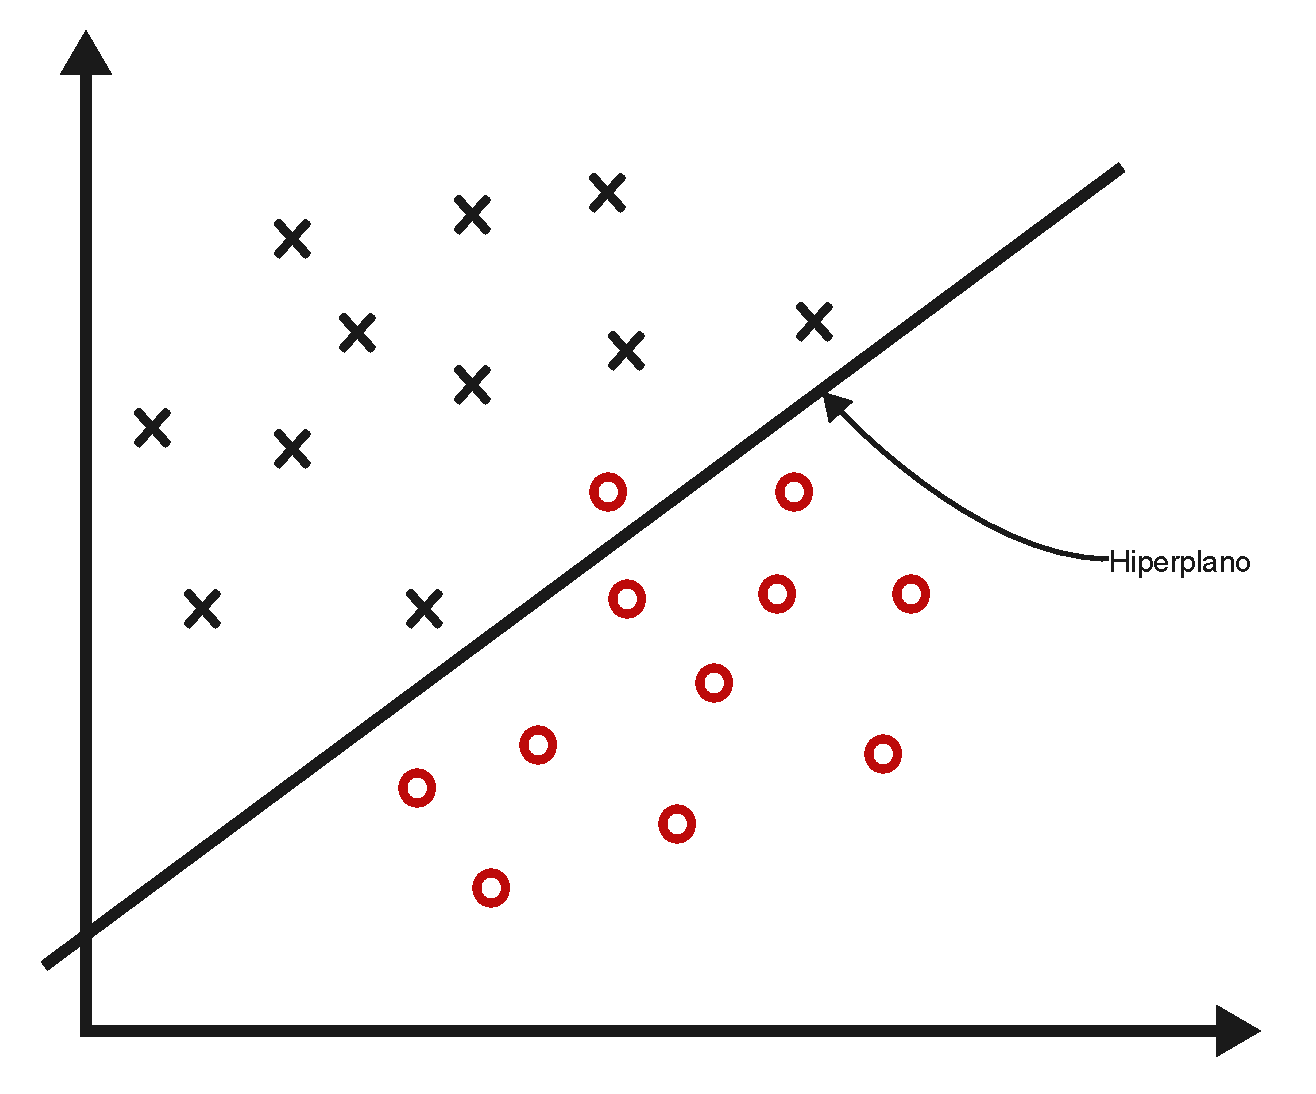
\includegraphics[width=0.6\textwidth]{images/hiperplano.pdf}
    \caption{Ejemplo bidimensional de un hiperplano que separa dos clases linealmente separables: las cruces negras pertenecen a una clase y los círculos rojos a la otra.}
    \label{fig:hiperplano_clasificacion}
\end{figure}

\section{Redes neuronales feedforward}

\subsection{Capas densas y notación matricial}

Una \textbf{capa densa} (o \textit{fully-connected}) agrupa muchas neuronas en paralelo. Sea $x \in \R^{d_{\text{in}}}$ la entrada a la capa. Una capa densa con $d_{\text{out}}$ neuronas se define como:
\begin{equation}
    z = W x + b, \quad z \in \R^{d_{\text{out}}},
\end{equation}
\begin{equation}
    y = \phi(z),
\end{equation}
donde:
\begin{itemize}
    \item $W \in \R^{d_{\text{out}} \times d_{\text{in}}}$ es la matriz de pesos.
    \item $b \in \R^{d_{\text{out}}}$ es el vector de sesgo.
    \item $\phi$ se aplica componente a componente. ($\phi: \R^{d_{\text{out}}} \to \R^{d_{\text{out}}}$, donde $\phi(z)=(\phi(z_i))_i$)
\end{itemize}

Para un conjunto de $N$ ejemplos, se suele apilar las entradas en una matriz $X \in \R^{N \times d_{\text{in}}}$ y la salida en $Y \in \R^{N \times d_{\text{out}}}$.

\subsection{Composición de capas}

Una \textbf{red neuronal feedforward} (o \textit{Multilayer Perceptron}, MLP) consiste en la composición de varias capas de este tipo. Por ejemplo, con dos capas ocultas:
\begin{align}
    h_1 &= \phi_1(W_1 x + b_1), \\
    h_2 &= \phi_2(W_2 h_1 + b_2), \\
    \hat{y} &= W_3 h_2 + b_3, \qquad \hat{y} \in \R^{d_{\text{out}}},
\end{align}

donde:
\begin{itemize}
    \item $x$ es la entrada.
    \item $h_1, h_2$ son representaciones internas (\textit{features} aprendidas).
    \item $\hat{y}$ es la salida del modelo (por ejemplo, una predicción de la serie de tiempo).
\end{itemize}

Este esquema se generaliza a un número arbitrario de capas. La capacidad de aproximación universal de las redes neuronales feedforward (bajo condiciones suaves sobre las funciones de activación) asegura que, con suficiente ancho y profundidad, pueden aproximar funciones muy complejas.

\begin{figure}[H]
    \centering
    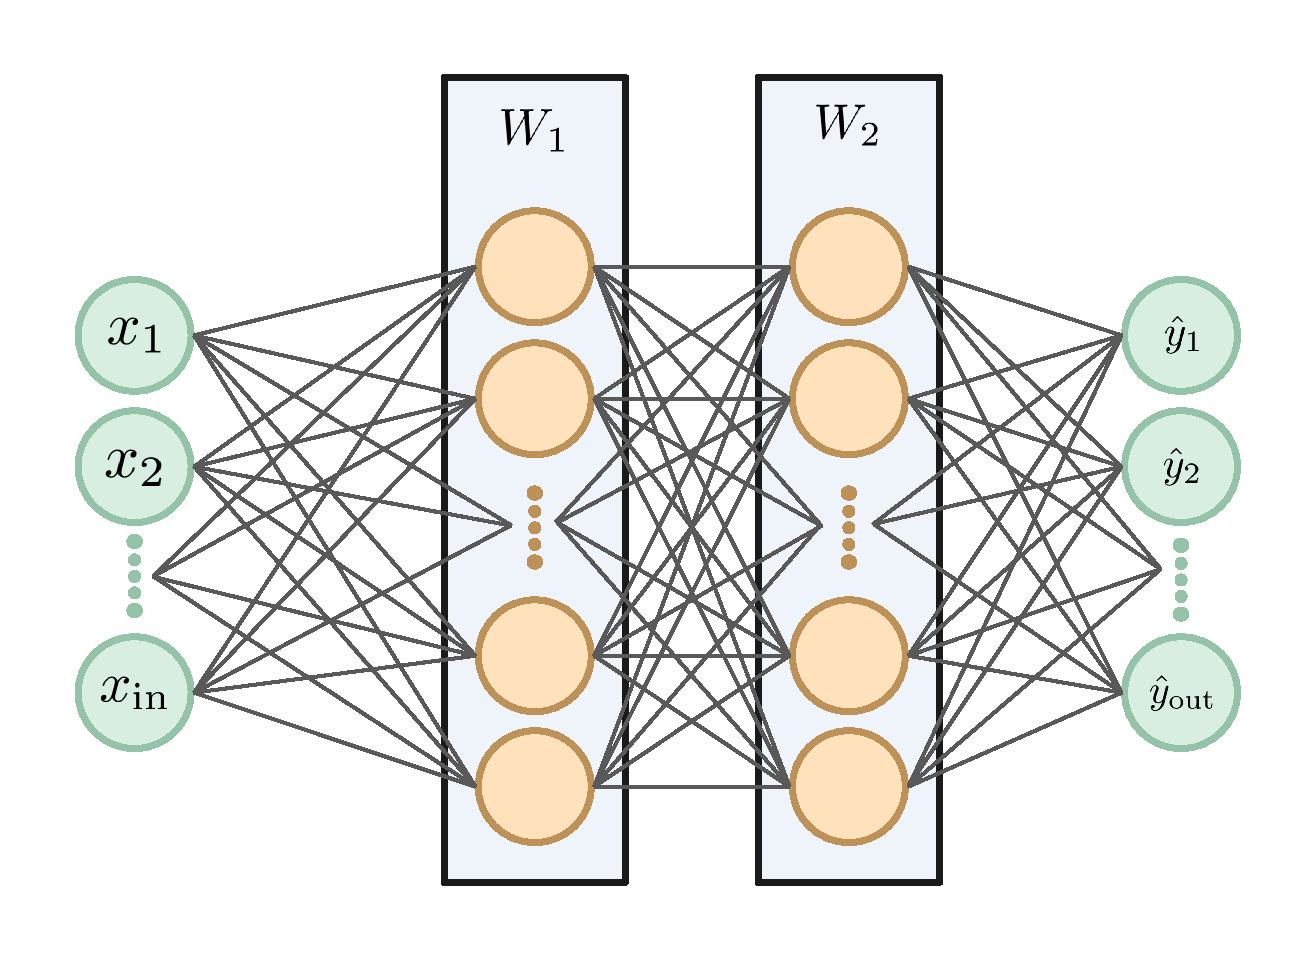
\includegraphics[width=0.6\textwidth]{images/Red neuronal.pdf}
    \caption{Esquema de una red neuronal \textit{feedforward} con dos capas ocultas: los vectores de entrada $x_1,\dots,x_{\text{in}}$ se transforman mediante las matrices de pesos $W_1$ y $W_2$ en representaciones internas, para finalmente producir las salidas $\hat{y}_1, \hat{y}_2, \dots, \hat{y}_{\text{out}}$.}
    \label{fig:red_mlp_dos_capas}
\end{figure}

\section{Función de pérdida}

\subsection{Pérdida para problemas de regresión}

En esta memoria el problema principal es de \textbf{regresión}: se quiere predecir un valor continuo (por ejemplo, el valor de una serie de tiempo en un instante futuro). Sea $\hat{y}_i$ la predicción del modelo para el ejemplo $i$ y $y_i$ el valor real. La función de pérdida más habitual es el \textbf{error cuadrático medio} (\textit{Mean Squared Error}, MSE):
\begin{equation}
    \mathcal{L}_{\text{MSE}}(\theta)
    = \frac{1}{N} \sum_{i=1}^{N} \|\hat{y}_i - y_i\|^2,
\end{equation}
donde $\theta$ representa el conjunto de todos los parámetros del modelo (todas las matrices $W$ y vectores $b$).

\hfill

El objetivo del entrenamiento es encontrar $\theta$ que minimice esta función de pérdida sobre el conjunto de datos de entrenamiento.

\hfill

Otras pérdidas útiles son, por ejemplo:
\begin{itemize}
    \item \textbf{Error absoluto medio} (MAE):
    \[
        \mathcal{L}_{\text{MAE}}(\theta)
        = \frac{1}{N} \sum_{i=1}^{N} \|\hat{y}_i - y_i\|_1.
    \]
    \item \textbf{Pérdida de Huber}, que combina propiedades de MSE y MAE, siendo más robusta a outliers.
\end{itemize}

\subsection{Regularización en la función de pérdida}

Para evitar sobreajuste (\textit{overfitting}), a menudo se agrega un término de \textbf{regularización} a la pérdida. Por ejemplo, regularización $L_2$ (también conocida como \textit{weight decay}):
\begin{equation}
    \mathcal{L}_{\text{total}}(\theta)
    = \mathcal{L}_{\text{datos}}(\theta)
    + \lambda \sum_{j} \|W_j\|_F^2,
\end{equation}
donde $\lambda > 0$ controla la fuerza de la regularización, y la suma recorre las matrices de pesos $W_j$ de cada capa.

\section{Descenso de gradiente y retropropagación}

\subsection{Descenso de gradiente}

El procedimiento básico para ajustar los parámetros de la red consiste en aplicar \textbf{descenso de gradiente}. Dada una función de pérdida $\mathcal{L}(\theta)$, el descenso de gradiente estándar actualiza los parámetros según:
\begin{equation}
    \theta_{t+1} = \theta_t - \eta \, \nabla_{\theta} \mathcal{L}(\theta_t),
\end{equation}
donde:
\begin{itemize}
    \item $\theta_t$ es el vector de parámetros en el paso $t$.
    \item $\eta > 0$ es la tasa de aprendizaje (\textit{learning rate}).
    \item $\nabla_{\theta} \mathcal{L}(\theta_t)$ es el gradiente de la pérdida respecto de los parámetros.
\end{itemize}

En la práctica, los datasets suelen ser grandes, por lo que calcular el gradiente sobre todos los datos en cada paso es costoso. Por ello se utiliza \textbf{descenso de gradiente estocástico} (SGD) o variantes \textit{mini-batch}, en las que el gradiente se estima a partir de un subconjunto de ejemplos:
\begin{equation}
    \theta_{t+1} = \theta_t - \eta \, \nabla_{\theta} \mathcal{L}_\mathcal{B}(\theta_t),
\end{equation}
donde $\mathcal{B}$ es un mini-batch de índices de entrenamiento.

\subsection{Retropropagación (\textit{backpropagation})}

Para poder aplicar descenso de gradiente, se requiere calcular el gradiente de la pérdida respecto de todos los parámetros de la red. Esto se logra mediante el algoritmo de \textbf{retropropagación}, que se basa en la regla de la cadena del cálculo diferencial.

\hfill

A nivel conceptual, la red se puede ver como una composición de funciones:
\begin{equation}
    \hat{y} = f_L \circ f_{L-1} \circ \cdots \circ f_1(x; \theta),
\end{equation}
donde cada $f_\ell$ representa una capa y depende de un subconjunto de parámetros $\theta_\ell$.

La regla de la cadena indica que:
\begin{equation}
    \frac{\partial \mathcal{L}}{\partial \theta_\ell}
    = \frac{\partial \mathcal{L}}{\partial f_\ell} \cdot 
      \frac{\partial f_\ell}{\partial \theta_\ell},
\end{equation}
y que las derivadas $\frac{\partial \mathcal{L}}{\partial f_\ell}$ se pueden calcular recursivamente desde la salida hacia la entrada.

\hfill

En términos prácticos:
\begin{enumerate}
    \item \textbf{Paso forward:} se propaga la entrada a través de la red y se calcula la pérdida.
    \item \textbf{Paso backward:} se calcula el gradiente de la pérdida respecto de la salida y se va propagando hacia atrás, capa por capa, acumulando las derivadas parciales.
    \item \textbf{Actualización:} se actualizan los parámetros usando el gradiente calculado y el algoritmo de optimización elegido (SGD, Adam, etc.).
\end{enumerate}

En frameworks modernos como PyTorch, este proceso se implementa automáticamente mediante \textit{autograd}, siempre que las operaciones definidas en el modelo sean diferenciables.

\section{Funciones de activación}

\subsection{Requisitos básicos}

La función de activación $\phi$ cumple dos roles fundamentales:
\begin{itemize}
    \item Introducir \textbf{no linealidad}. Sin funciones de activación, la composición de capas lineales sigue siendo una transformación lineal global.
    \item Ser \textbf{diferenciable} (al menos por tramos) para poder aplicar retropropagación.
\end{itemize}

A continuación se describen algunas de las funciones de activación más utilizadas.

\subsection{Sigmoide y tangente hiperbólica}

La función \textbf{sigmoide} se define como:
\begin{equation}
    \sigma(z) = \frac{1}{1 + e^{-z}}.
\end{equation}
Sus valores están en el intervalo $(0, 1)$ y su derivada es:
\begin{equation}
    \sigma'(z) = \sigma(z) \, (1 - \sigma(z)).
\end{equation}

La \textbf{tangente hiperbólica} se define como:
\begin{equation}
    \tanh(z) = \frac{e^{z} - e^{-z}}{e^{z} + e^{-z}},
\end{equation}
con valores en $(-1, 1)$ y derivada:
\begin{equation}
    \tanh'(z) = 1 - \tanh^2(z).
\end{equation}

Ambas funciones se usaron ampliamente en redes neuronales clásicas, pero presentan el problema de \textbf{gradientes que se desvanecen} (\textit{vanishing gradients}) para valores de $|z|$ grandes, lo que dificulta el entrenamiento de redes profundas.

\subsection{ReLU y variantes}

La \textbf{Rectified Linear Unit} (ReLU) se define como:
\begin{equation}
    \mathrm{ReLU}(z) = \max(0, z).
\end{equation}
Su derivada es:
\[
    \mathrm{ReLU}'(z) =
    \begin{cases}
        1, & z > 0, \\
        0, & z \le 0.
    \end{cases}
\]

Las ReLU han sido muy exitosas en redes profundas porque mitigan parcialmente el problema de gradientes que se desvanecen en la región $z > 0$ y son computacionalmente simples. Sin embargo, pueden producir neuronas ``muertas'' (salida cero constante) si los pesos se actualizan de forma que $z$ permanezca en la región negativa.

\hfill

Variantes como \textbf{Leaky ReLU} introducen un pequeño gradiente en la región negativa:
\[
    \mathrm{LeakyReLU}(z) =
    \begin{cases}
        z, & z > 0, \\
        \alpha z, & z \le 0,
    \end{cases}
\]
con $\alpha$ pequeño (por ejemplo, $\alpha = 0{,}01$).

\hfill

En modelos más recientes, incluyendo Transformers, es frecuente usar activaciones más suaves como \textbf{GELU} (\textit{Gaussian Error Linear Unit}), que puede verse como una versión suavizada de ReLU con ciertas propiedades teóricas favorables.

\section{Problemas en el entrenamiento de redes profundas}

\subsection{Gradientes que se desvanecen y explotan}

En redes profundas, al aplicar retropropagación, se multiplican muchas matrices y derivadas de funciones de activación. Esto puede llevar a que:
\begin{itemize}
    \item Los gradientes se hagan extremadamente pequeños (\textbf{vanishing gradients}), dificultando el aprendizaje en capas tempranas.
    \item Los gradientes crezcan de forma descontrolada (\textbf{exploding gradients}), causando inestabilidad numérica.
\end{itemize}

Existen varias estrategias para mitigar estos problemas:
\begin{itemize}
    \item Diseñar buenas \textbf{inicializaciones} de los pesos (por ejemplo, He o Xavier).
    \item Utilizar funciones de activación adecuadas (ReLU, GELU, etc.).
    \item Aplicar \textbf{normalizaciones}, como \textit{Batch Normalization} o \textit{Layer Normalization}.
    \item Aplicar \textbf{clipping de gradiente}, limitando la norma del gradiente en cada actualización.
\end{itemize}

\subsection{Regularización y generalización}

Además de los términos de regularización en la pérdida, existen técnicas adicionales para mejorar la capacidad de generalización:
\begin{itemize}
    \item \textbf{Dropout}: durante el entrenamiento, se anulan aleatoriamente algunas neuronas (se ponen a cero) con cierta probabilidad, lo que fuerza al modelo a no depender excesivamente de un subconjunto pequeño de unidades.
    \item \textbf{Early stopping}: se detiene el entrenamiento cuando la pérdida de validación deja de mejorar, evitando sobreajuste.
    \item \textbf{Data augmentation}: en dominios como imágenes o texto, se generan ejemplos adicionales modificando ligeramente los datos originales. En series de tiempo esto es más delicado, pero existen técnicas específicas.
\end{itemize}

\section{Optimizadores avanzados: Adam}

\subsection{Motivación}

El descenso de gradiente estándar utiliza una única tasa de aprendizaje $\eta$ para todos los parámetros y no tiene memoria explícita del historial de gradientes. En problemas complejos y de alta dimensión, esto puede hacer que:
\begin{itemize}
    \item El entrenamiento sea sensible a la elección de $\eta$.
    \item El modelo tarde en converger o quede atrapado en regiones poco favorables.
\end{itemize}

Por ello se han desarrollado \textbf{optimizadores avanzados} que adaptan la tasa de aprendizaje de manera automática, utilizando información adicional sobre la historia del gradiente. Uno de los más usados en la práctica es \textbf{Adam} (\textit{Adaptive Moment Estimation}).

\subsection{Algoritmo Adam}

Sea $\theta_t$ el vector de parámetros en el paso $t$ y $g_t = \nabla_\theta \mathcal{L}_t(\theta_t)$ el gradiente de la pérdida calculado en ese paso (por ejemplo, sobre un mini-batch). Adam mantiene dos variables auxiliares:
\begin{itemize}
    \item $m_t$: estimación del primer momento (media) del gradiente.
    \item $v_t$: estimación del segundo momento (varianza no centrada) del gradiente.
\end{itemize}

El algoritmo puede describirse como sigue:

\begin{enumerate}
    \item Inicializar $m_0 = 0$, $v_0 = 0$, $t = 0$.
    \item En cada paso:
    \begin{align}
        t &\leftarrow t + 1, \\
        g_t &\leftarrow \nabla_\theta \mathcal{L}_t(\theta_t), \\
        m_t &\leftarrow \beta_1 m_{t-1} + (1 - \beta_1) g_t, \\
        v_t &\leftarrow \beta_2 v_{t-1} + (1 - \beta_2) g_t^2,
    \end{align}
    donde las operaciones son componente a componente y $0 < \beta_1, \beta_2 < 1$ son hiperparámetros (típicamente $\beta_1 \approx 0{,}9$, $\beta_2 \approx 0{,}999$).
    \item Para corregir el sesgo inicial (ya que $m_t$ y $v_t$ parten en cero), se calculan:
    \begin{align}
        \hat{m}_t &= \frac{m_t}{1 - \beta_1^{t}}, \\
        \hat{v}_t &= \frac{v_t}{1 - \beta_2^{t}}.
    \end{align}
    \item Finalmente, se actualizan los parámetros:
    \begin{equation}
        \theta_{t+1}
        = \theta_t - \eta \, \frac{\hat{m}_t}{\sqrt{\hat{v}_t} + \varepsilon},
    \end{equation}
    donde $\eta$ es la tasa de aprendizaje base y $\varepsilon$ es un pequeño valor positivo (por ejemplo, $10^{-8}$) para evitar divisiones por cero.
\end{enumerate}

En palabras simples:
\begin{itemize}
    \item $m_t$ actúa como un \textbf{promedio móvil} del gradiente (similar a \textit{momentum}).
    \item $v_t$ actúa como un promedio móvil de la magnitud cuadrática del gradiente, permitiendo \textbf{adaptar} la escala de los pasos por parámetro.
    \item La división por $\sqrt{\hat{v}_t}$ hace que los parámetros con gradientes consistentemente grandes tengan pasos de actualización más pequeños, y viceversa.
\end{itemize}

En esta memoria se utiliza AdamW como optimizador principal para entrenar los modelos Transformer, tal como se especifica en los archivos de configuración de entrenamiento. AdamW conserva el carácter adaptativo de Adam, pero desacopla el decaimiento de pesos de la actualización basada en momentos.

\section{Relación con \CTTransformer}

Aunque el Transformer parece, a primera vista, una arquitectura muy distinta a un MLP estándar, en el fondo reutiliza los mismos componentes básicos descritos en este anexo:

\begin{itemize}
    \item Cada bloque de \textbf{atención multi-cabeza} está compuesto por proyecciones lineales (capas densas) que calculan las matrices de \textit{queries}, \textit{keys} y \textit{values}, seguidas de operaciones de atención y una proyección lineal de salida.
    \item El \textbf{bloque feed-forward} dentro de cada capa del Transformer es esencialmente un MLP de dos capas aplicado posición a posición, con una función de activación no lineal (por ejemplo, ReLU o GELU).
    \item La red completa se entrena minimizando una función de pérdida (en este caso, típicamente MSE sobre las predicciones de la serie de tiempo) usando descenso de gradiente y un optimizador como Adam o AdamW.
    \item La \textbf{cabeza de regresión} sobre el token \textit{target} en el modelo de esta memoria es, nuevamente, una capa lineal (o una pequeña MLP) que transforma la representación latente del token en la predicción final.
\end{itemize}

Por lo tanto, comprender el funcionamiento de neuronas, funciones de activación, retropropagación y optimizadores adaptativos como Adam o AdamW es suficiente para entender el entrenamiento de toda la arquitectura \CTTransformer, aunque los detalles de la atención, los encodings temporales y el scheduler usado en los experimentos se desarrollen en capítulos específicos y en el Anexo~\ref{anexo:optimizacion-scheduler}.

\section{Resumen del anexo}

En este anexo se han presentado los fundamentos necesarios para comprender el entrenamiento de redes neuronales modernas:
\begin{itemize}
    \item El modelo de neurona artificial como combinación lineal más función de activación.
    \item La construcción de redes feedforward mediante la composición de capas densas.
    \item La definición de funciones de pérdida para problemas de regresión y el uso de regularización.
    \item El algoritmo de entrenamiento basado en descenso de gradiente, estimado mediante mini-batches, y el cálculo eficiente de gradientes mediante retropropagación.
    \item El rol de las funciones de activación y los problemas asociados al entrenamiento de redes profundas (gradientes que se desvanecen o explotan).
    \item El algoritmo Adam y su variante AdamW como optimizadores adaptativos ampliamente utilizados en la práctica.
\end{itemize}

Estos conceptos constituyen la base sobre la cual se construyen las arquitecturas específicas analizadas en la memoria, en particular \CTTransformer.
